\documentclass[11pt,english]{article}\usepackage[]{graphicx}\usepackage{xcolor}
% maxwidth is the original width if it is less than linewidth
% otherwise use linewidth (to make sure the graphics do not exceed the margin)
\makeatletter
\def\maxwidth{ %
  \ifdim\Gin@nat@width>\linewidth
    \linewidth
  \else
    \Gin@nat@width
  \fi
}
\makeatother

\definecolor{fgcolor}{rgb}{0.345, 0.345, 0.345}
\newcommand{\hlnum}[1]{\textcolor[rgb]{0.686,0.059,0.569}{#1}}%
\newcommand{\hlstr}[1]{\textcolor[rgb]{0.192,0.494,0.8}{#1}}%
\newcommand{\hlcom}[1]{\textcolor[rgb]{0.678,0.584,0.686}{\textit{#1}}}%
\newcommand{\hlopt}[1]{\textcolor[rgb]{0,0,0}{#1}}%
\newcommand{\hlstd}[1]{\textcolor[rgb]{0.345,0.345,0.345}{#1}}%
\newcommand{\hlkwa}[1]{\textcolor[rgb]{0.161,0.373,0.58}{\textbf{#1}}}%
\newcommand{\hlkwb}[1]{\textcolor[rgb]{0.69,0.353,0.396}{#1}}%
\newcommand{\hlkwc}[1]{\textcolor[rgb]{0.333,0.667,0.333}{#1}}%
\newcommand{\hlkwd}[1]{\textcolor[rgb]{0.737,0.353,0.396}{\textbf{#1}}}%
\let\hlipl\hlkwb

\usepackage{framed}
\makeatletter
\newenvironment{kframe}{%
 \def\at@end@of@kframe{}%
 \ifinner\ifhmode%
  \def\at@end@of@kframe{\end{minipage}}%
  \begin{minipage}{\columnwidth}%
 \fi\fi%
 \def\FrameCommand##1{\hskip\@totalleftmargin \hskip-\fboxsep
 \colorbox{shadecolor}{##1}\hskip-\fboxsep
     % There is no \\@totalrightmargin, so:
     \hskip-\linewidth \hskip-\@totalleftmargin \hskip\columnwidth}%
 \MakeFramed {\advance\hsize-\width
   \@totalleftmargin\z@ \linewidth\hsize
   \@setminipage}}%
 {\par\unskip\endMakeFramed%
 \at@end@of@kframe}
\makeatother

\definecolor{shadecolor}{rgb}{.97, .97, .97}
\definecolor{messagecolor}{rgb}{0, 0, 0}
\definecolor{warningcolor}{rgb}{1, 0, 1}
\definecolor{errorcolor}{rgb}{1, 0, 0}
\newenvironment{knitrout}{}{} % an empty environment to be redefined in TeX

\usepackage{alltt} 

\usepackage[a4paper]{geometry}
% \usepackage{fullpage}
\usepackage{natbib}
\usepackage{algorithm}
\usepackage{graphicx}

% \usepackage{mathptmx}
\usepackage{alphalph}

\usepackage[utf8]{inputenc}
\usepackage[T1]{fontenc}
\usepackage{tikz}
\usepackage{float}

\usepackage[colorlinks = true,linkcolor = blue, citecolor = blue]{hyperref}
\usepackage{booktabs}
\usepackage{amssymb,amsmath}%,natbib,rotating,mfpic} %amsmath}


% \usepackage{layouts}

\def\aaa{a}
\def\aaag{\textbf{a}}
\def\R{\mathbb{R}}
\def\N{\mathbb{N}}
\def\tb{{\bf t}}
\def\zerog{{\bf 0}}
\def\trace{{\rm trace}}
\def\rang{{\rm rang}}
\def\Gammag{\mathbf{\Gamma}}
\def\Deltag{\mathbf{\Delta}}
\def\Thetag{\mathbf{\Theta}}
\def\Lambdag{\mathbf{\Lambda}}
\def\Xig{\mathbf{\Xi}}
\def\Pig{\mathbf{\Pi}}
\def\Sigmag{\mathbf{\Sigma}}
\def\Pig{\mathbf{\Pib}}
\def\Phig{\mathbf{\Phi}} %
\def\Psig{\mathbf{\Psi}} %}}
\def\Omegag{\mathbf{\Omega}} %}}
\def\Upsilong{\mathbf{\Upsilon}} %}}


\def\Var{{\rm var}}
\def\Min{{\rm Min}}
\def\Cov{{\rm cov}}
\def\Corr{{\rm corr}}
\def\Im{{\rm Im}}
\def\Ker{{\rm Ker}}
\def\SC{{\rm SC}}
\def\CM{{\rm CM}}
\def\diag{{\rm diag}}
\def\E{{\rm E}}
\def\Pr{{\rm Pr}}
\def\Vb{{\bf V}}




%%%%%%%%%%%%%%%%%%%%%%%%%%%%%%%%%%%%%%%%%%%%%%%%%%%%%%
\def\alphag{\boldsymbol{\alpha}} %$\alpha$
\def\betag{\boldsymbol{\beta}} %$\beta$
\def\gammag{\boldsymbol{\gamma}} %$\gamma$
\def\deltag{\boldsymbol{\delta}} %$\delta$
\def\epsilong{\boldsymbol{\epsilon}} %$\epsilon$
\def\varepsilong{\boldsymbol{\varepsilon}} %$\varepsilon$
\def\etag{\boldsymbol{\eta}} %$\eta$
\def\thetag{\boldsymbol{\theta}} %$\theta$
\def\iotag{\boldsymbol{\iota}} %$\iota$
\def\kappag{\boldsymbol{\kappa}} %$\kappa$
\def\lambdag{\boldsymbol{\lambda}} %$\lambda$
\def\mug{\boldsymbol{\mu}} %$\nu$
\def\nug{\boldsymbol{\nu}} %$\mu$
\def\xig{\boldsymbol{\xi}} %$\xi$
\def\pig{\boldsymbol{\pi}} %$\pi$
\def\rhog{\boldsymbol{\rho}} %$\rho$
\def\sigmag{\boldsymbol{\sigma}} %$\sigma$
\def\taug{\boldsymbol{\tau}} %$\tau$
\def\upsilong{\boldsymbol{\upsilon}} %$\upsilon$
\def\phig{\boldsymbol{\phi}} %$\phi$
\def\chig{\boldsymbol{\chi}} %$\chi$
\def\psig{\boldsymbol{\psi}} %$\psi$
\def\omegag{\boldsymbol{\omega}} %$\omega$

%%%%%%%%%%%%%%%%%%%%%%%%%%%%%%%%%%%%%%%%%%%%%%%%%%%%%%

\def\tb{{\bf t}}
\def\zerog{{\bf 0}}
\def\trace{{\rm trace}}
\def\rang{{\rm rang}}
\def\Gammag{\mathbf{\Gamma}}
\def\Deltag{\mathbf{\Delta}}
%\def\Thetag{\mathbf{\Theta}}
\def\Lambdag{\mathbf{\Lambda}}
%\def\Xig{\mathbf{\Xi}}
%\def\Pig{\mathbf{\Pi}}
\def\Sigmag{\mathbf{\Sigma}}
%\def\Pig{\mathbf{\Pib}}
%\def\Phig{\mathbf{\Phi}} %
%\def\Psig{\mathbf{\Psi}} %}}
\def\Omegag{\mathbf{\Omega}} %}}


\def\Xbu{{\bf X}_1}
\def\Xbd{{\bf X}_2}
\def\Xbt{{\bf X}_3}
%\def\Yb{{\bf Y}}
\def\Db{{\bf D}}
\def\Eb{{\bf E}}
\def\Fb{{\bf F}}
\def\Tb{{\bf T}}

\def\nb{{\bf n}}
\def\ab{{\bf a}}
\def\sb{{\bf s}}
\def\eb{{\bf e}}
\def\gb{{\bf g}}
\def\rb{{\bf r}}
\def\cg{{\bf c}}

\def\yb{{\bf y}}
\def\zb{{\bf z}}
\def\bb{{\bf b}}
\def\cb{{\bf c}}
\def\fb{{\bf f}}
\def\ub{{\bf u}}
\def\xb{{\bf x}}
\def\vb{{\bf v}}
\def\wb{{\bf w}}
\def\Ab{{\bf A}}
\def\Bb{{\bf B}}
\def\Cb{{\bf C}}
\def\Mb{{\bf M}}
\def\Nb{{\bf N}}
\def\Cg{{\bf C}}
\def\Ib{{\bf I}}
\def\Xb{{\bf X}}
\def\Zb{{\bf Z}}
\def\Pb{{\bf P}}
\def\Db{{\bf D}}
\def\Rb{{\bf R}}
\def\Qb{{\bf Q}}
\def\Sb{{\bf S}}
\def\Ub{{\bf U}}
\def\Wb{{\bf W}}
\def\0b{{\bf 0}}
\def\1b{{\bf 1}}

\newtheorem{exmpl}{Example}[section]

\newcommand{\myalphafoot}
{
\renewcommand{\thefootnote}{\alph{footnote}}
}

\title{Statistical Analysis for Eukaryote}
\myalphafoot
\author{\myalphafoot Rapha\"el Jauslin\footnotemark[1]}
\date{}
\footnotetext[1]{Institute of statistics, University of Neuchatel, Av. de Bellevaux 51, 2000 Neuchatel, Switzerland\\ (E-mail: raphael.jauslin@unine.ch)}
\IfFileExists{upquote.sty}{\usepackage{upquote}}{}
\begin{document}


% \maketitle




\begin{abstract}
Statistical analysis of Eukaroyte data. The idea is to see whether diferent treatment have an effect of the biodiversity of the protist community in soils.\\
\textbf{Key words}: protist microbiome, cadaver, soils, V4 region of 18S rRNA
\end{abstract}

\newpage
\section{Introduction}


\section{Richness}




% \begin{figure}[ht!]
% \centering
% \input{shannon.tex}
% \caption{Protist OTU Richness and Shannon diverstiy}
% \label{fig:shan}
% \end{figure}








\begin{figure}[ht!]
\centering
\begin{knitrout}
\definecolor{shadecolor}{rgb}{0.969, 0.969, 0.969}\color{fgcolor}
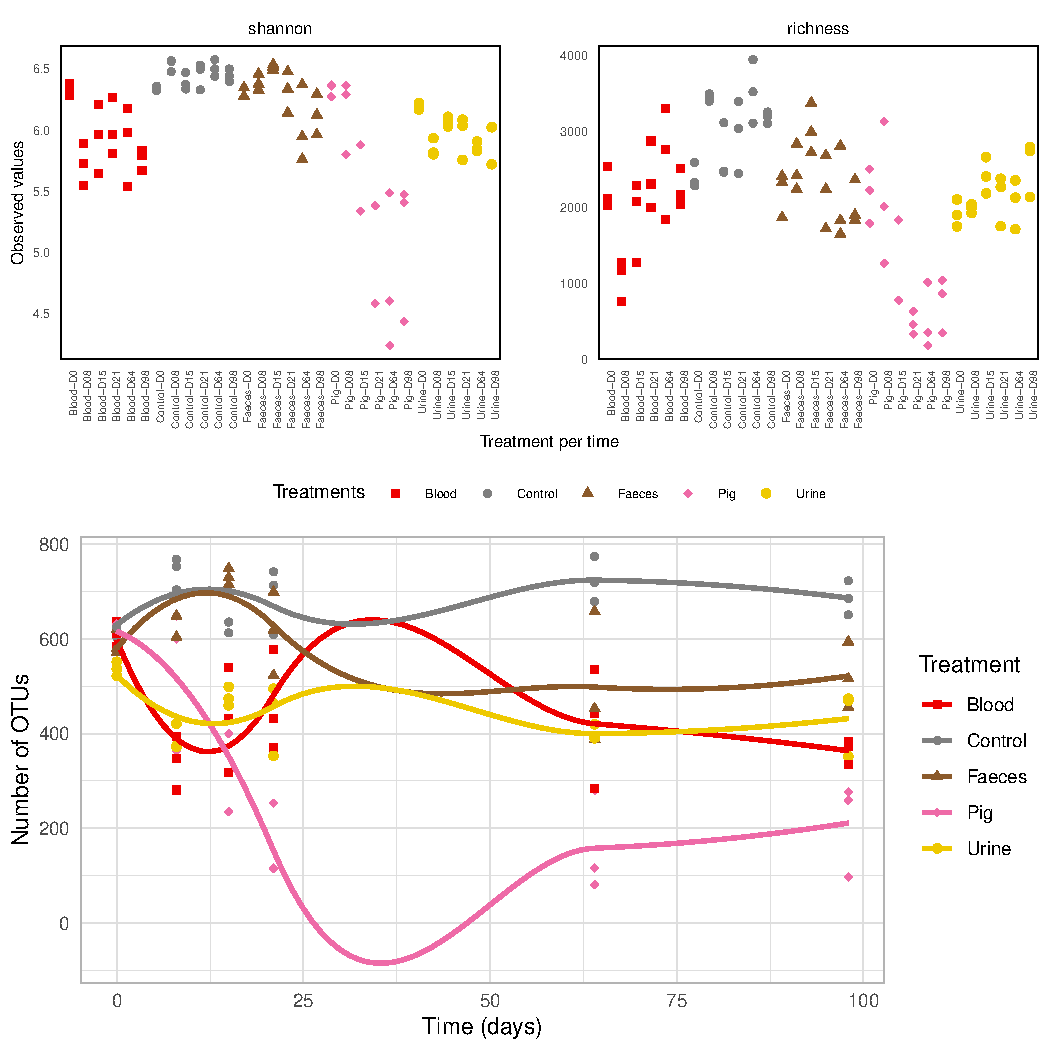
\includegraphics[width=\maxwidth]{figure/image-div-1} 

\end{knitrout}
\caption{Protist OTU diverstiy, presence-absence transform.}
\label{fig:loess}
\end{figure}

% \begin{figure}[ht!]
% \centering
% \input{loess.tex}
% \caption{Protist OTU diverstiy, presence-absence transform.}
% \label{fig:loess}
% \end{figure}



\begin{knitrout}
\definecolor{shadecolor}{rgb}{0.969, 0.969, 0.969}\color{fgcolor}
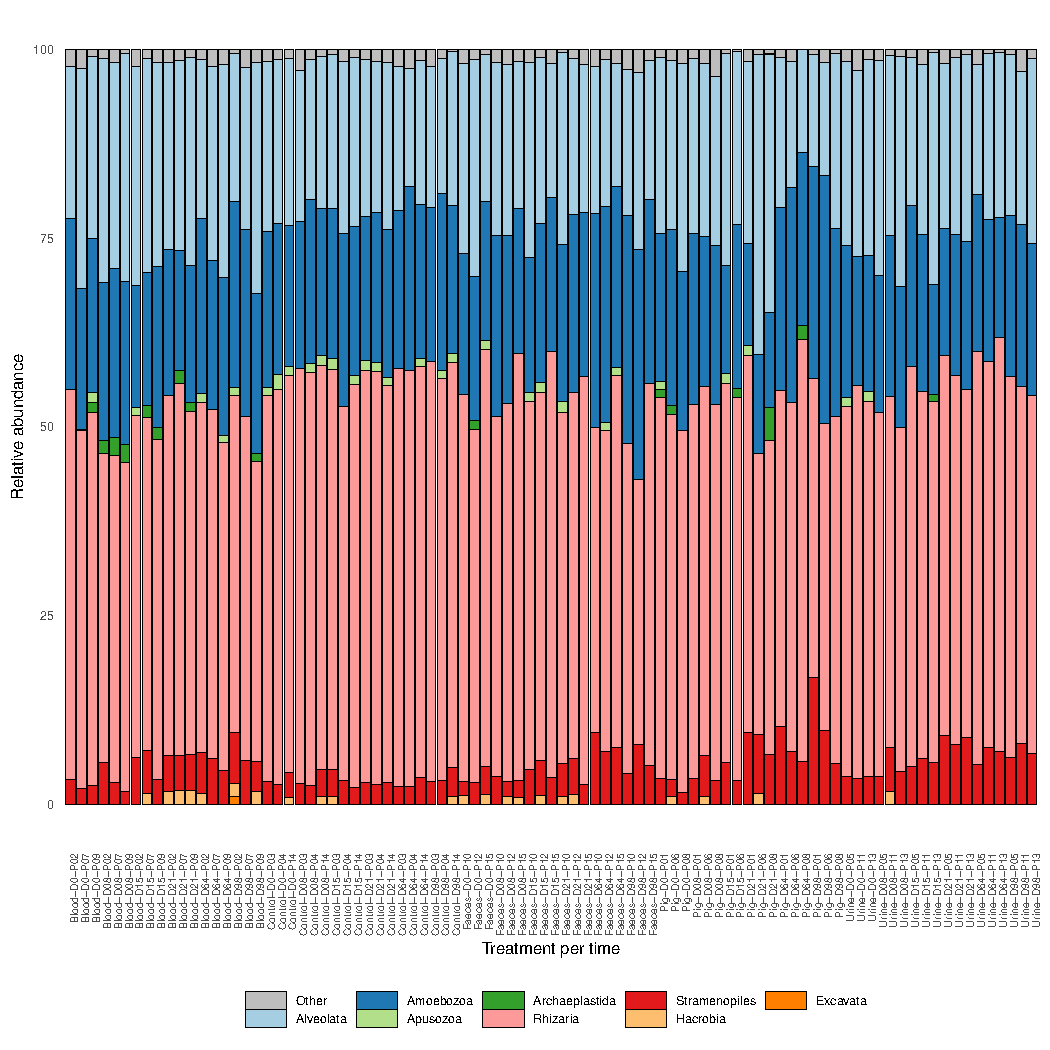
\includegraphics[width=\maxwidth]{figure/image-taxo_profile-1} 

\end{knitrout}


\section{NMDS}


\begin{knitrout}
\definecolor{shadecolor}{rgb}{0.969, 0.969, 0.969}\color{fgcolor}
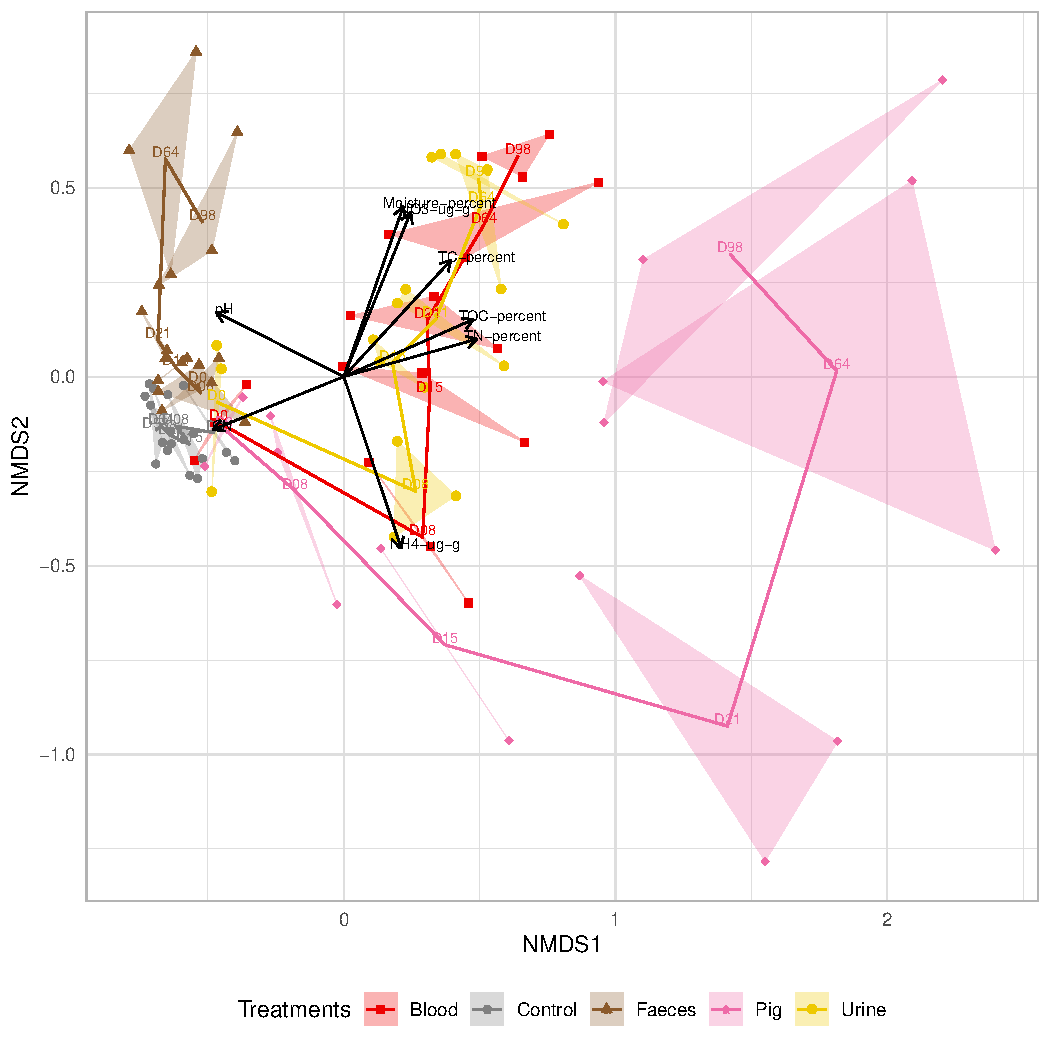
\includegraphics[width=\maxwidth]{figure/image-nmds-1} 

\end{knitrout}


\section{RDA}


\begin{knitrout}
\definecolor{shadecolor}{rgb}{0.969, 0.969, 0.969}\color{fgcolor}
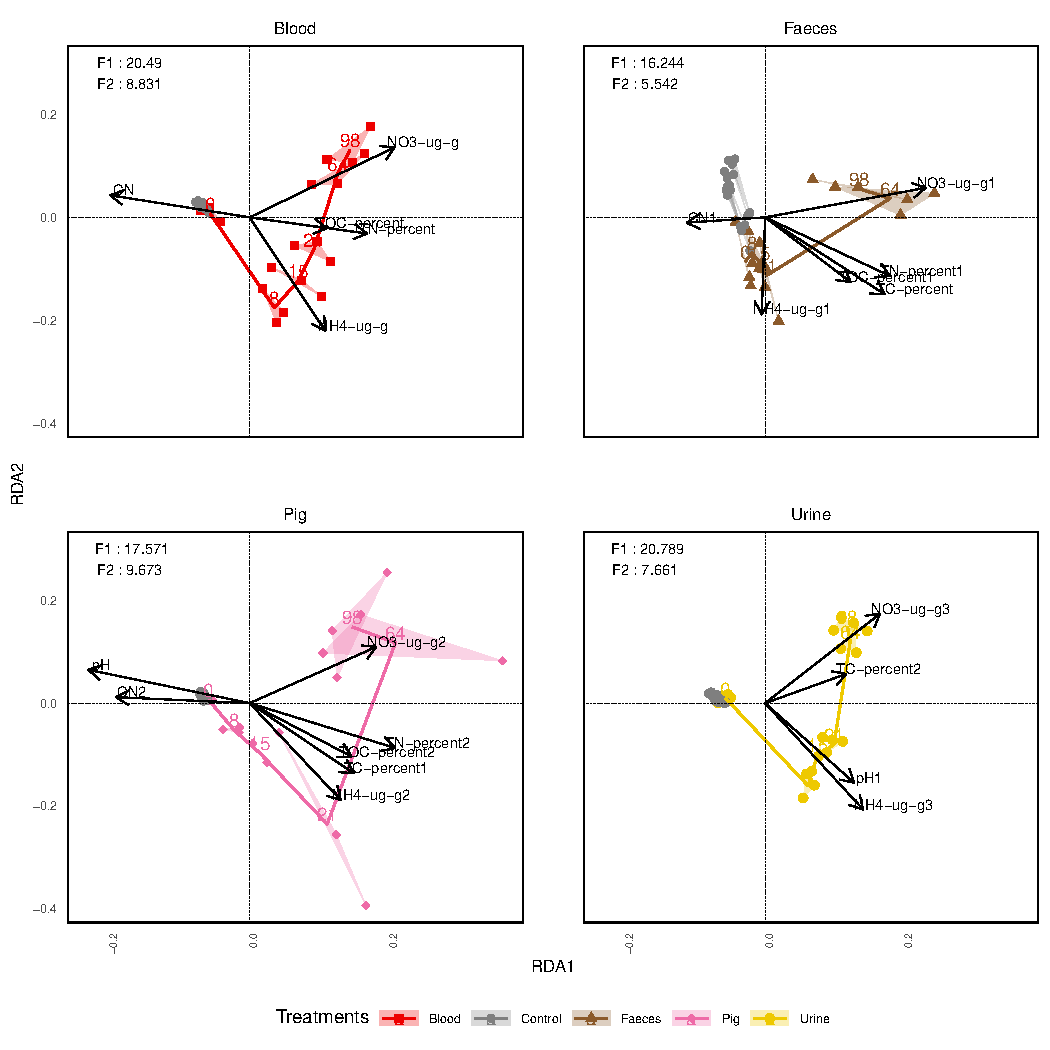
\includegraphics[width=\maxwidth]{figure/image-rda-1} 

\end{knitrout}

% \begin{figure}[ht!]
% \centering
% \input{rda.tex}
% \caption{Redundancy analysis (RDA).}
% \label{fig:da}
% \end{figure}






\section{Bioindicator}

\begin{knitrout}
\definecolor{shadecolor}{rgb}{0.969, 0.969, 0.969}\color{fgcolor}
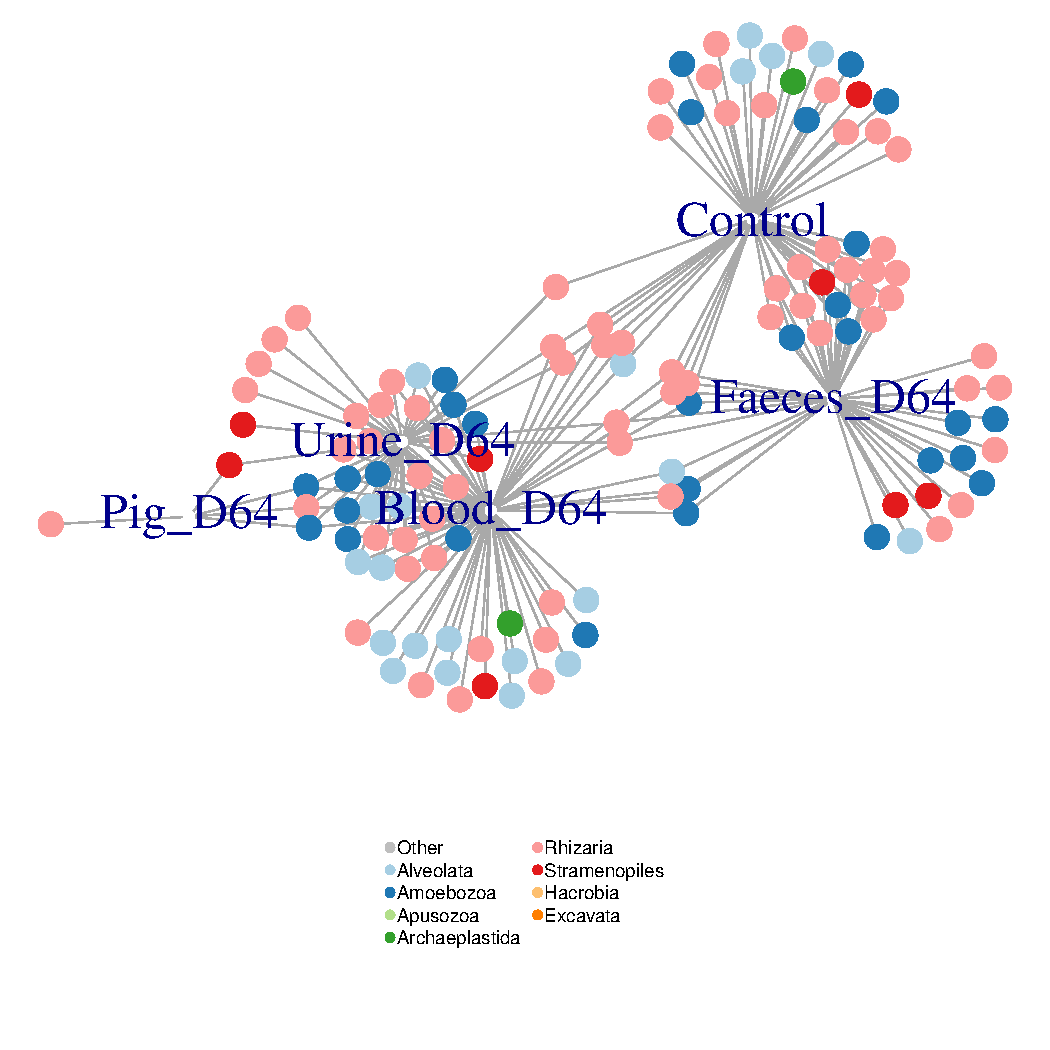
\includegraphics[width=\maxwidth]{figure/image-bioindic-1} 

\end{knitrout}

\section{Heatmap}

\begin{knitrout}
\definecolor{shadecolor}{rgb}{0.969, 0.969, 0.969}\color{fgcolor}
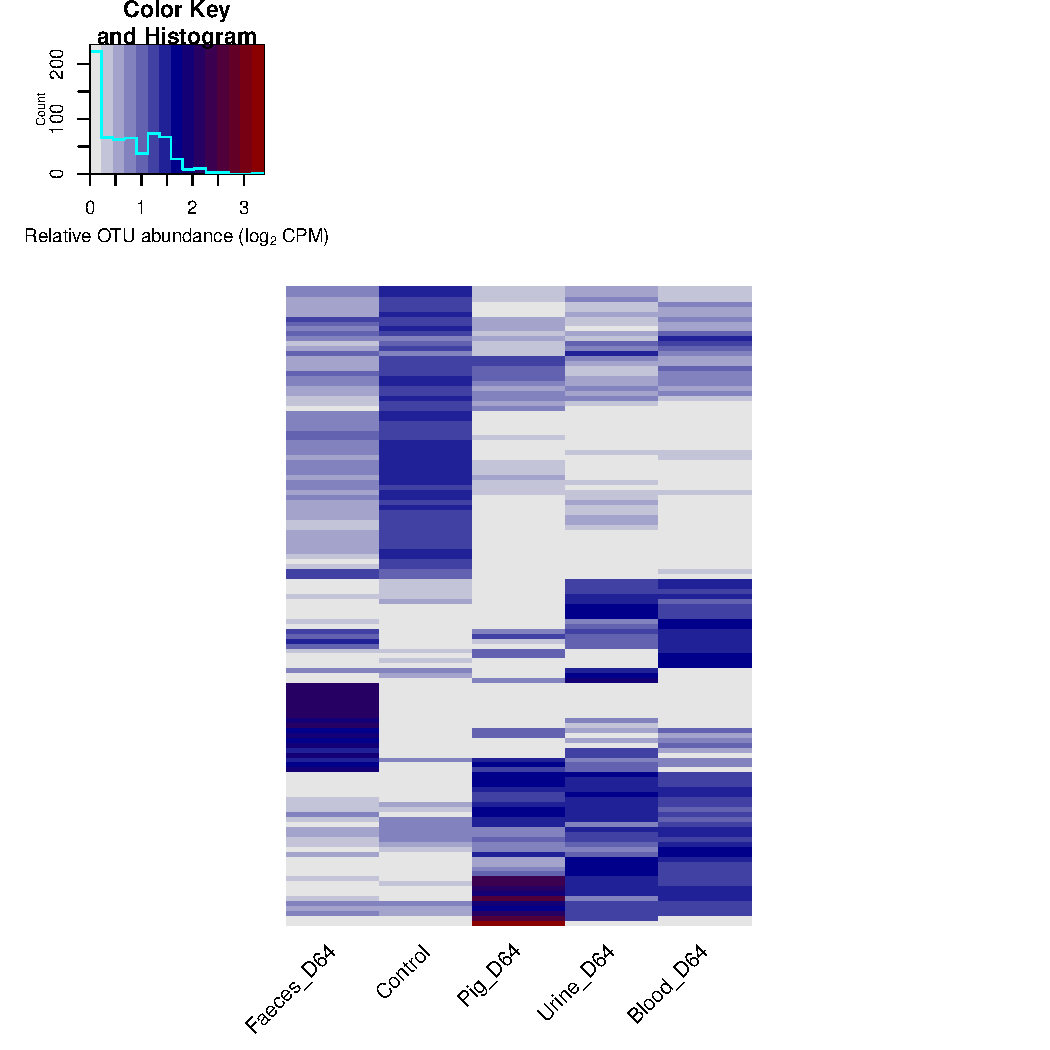
\includegraphics[width=\maxwidth]{figure/image-heatmap-1} 

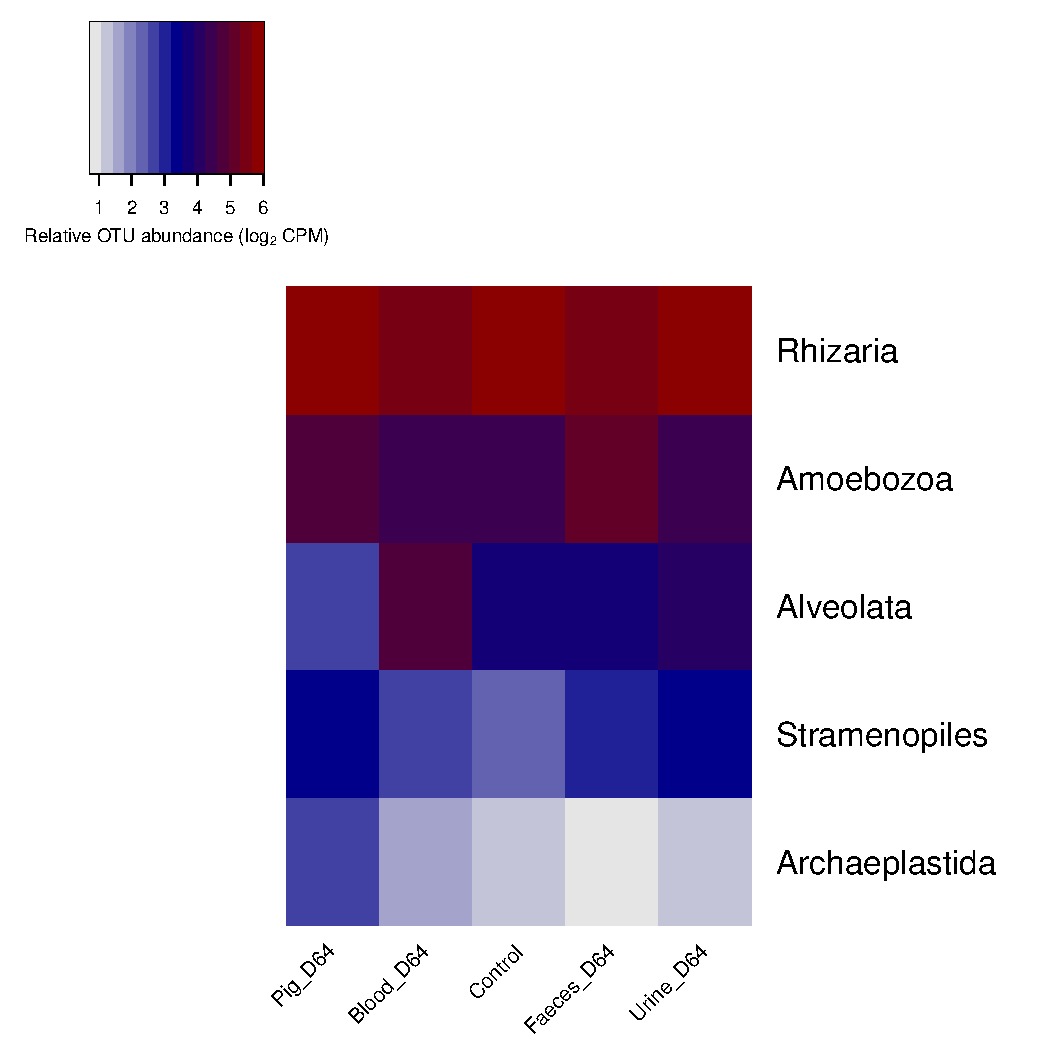
\includegraphics[width=\maxwidth]{figure/image-heatmap-2} 

\end{knitrout}

% \bibliography{bibyves}
% \bibliographystyle{apalike}

\end{document}
